\documentclass[12pt,fleqn]{article}\usepackage{../../common}
\begin{document}
Derin ��renme ile Oyun Oynamak, AlphaGo Zero, DeepMind











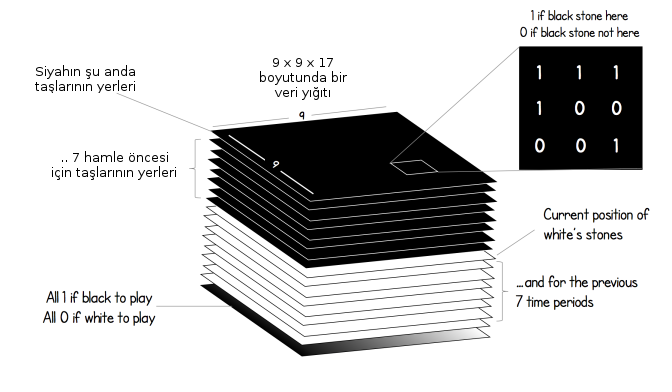
\includegraphics[width=30em]{go_01.png}


\inputminted[fontsize=\footnotesize]{python}{mcts.py}


\inputminted[fontsize=\footnotesize]{python}{train.py}

\inputminted[fontsize=\footnotesize]{python}{simplenet.py}



Kaynaklar

[1] {\em Go Oyun Kurallar�}, \url{https://www.dropbox.com/s/xfcimo9ojhq3l2l/go.pdf?dl=1}

[2] Silver, {\em Mastering the game of Go with deep neural networks and tree search}, \url{https://www.nature.com/articles/nature16961}

[3] Weidman, {\em The 3 Tricks That Made AlphaGo Zero Work}, \url{https://hackernoon.com/the-3-tricks-that-made-alphago-zero-work-f3d47b6686ef}

[4] Yi, {\em A reproduction of Alphago Zero in 'Mastering the game of Go without human knowledge'}, \url{https://github.com/sangyi92/alphago_zero}

[5] {\em AlphaGo Zero Cheat Sheet}, \url{https://applied-data.science/static/main/res/alpha_go_zero_cheat_sheet.png}

\end{document}
